% ==============================================================================
% BÁO CÁO KỸ THUẬT: KIỂM TRA TÍNH TIN CẬY MÔ HÌNH TINY-MOBILEFACENET
% Tác giả: Nguyễn Sỹ Tuấn Anh
% Ngày cập nhật: 22/11/2026
% Hướng dẫn biên dịch:
% 1. Trên Overleaf: Tạo project mới, tải file .tex và ảnh lfw_benchmark_report.png lên,
%    chọn trình biên dịch pdfLaTeX (mặc định) hoặc XeLaTeX.
% 2. Trên máy tính cục bộ: pdflatex Kiem_Tra_Tinh_Tin_Cay_TinyMobileFaceNet.tex
% ==============================================================================

\documentclass[11pt,a4paper]{article}

% --- Gói ngôn ngữ & Bảng mã tiếng Việt ---
\usepackage[utf8]{inputenc}
\usepackage[vietnamese]{babel}
\usepackage[margin=2.1cm]{geometry}

% --- Gói toán học & Ký hiệu ---
\usepackage{amsmath,amssymb,amsfonts}

% --- Gói đồ họa & Bảng biểu ---
\usepackage{graphicx}
\usepackage{booktabs}
\usepackage{array}
\usepackage{float}
\usepackage{caption}

% --- Gói định dạng Code Python ---
\usepackage{listings}
\usepackage{xcolor}

% --- Gói liên kết & Tham chiếu ---
\usepackage{hyperref}
\hypersetup{
    colorlinks=true,
    linkcolor=blue!80!black,
    citecolor=blue!80!black,
    urlcolor=teal
}

% Cấu hình hiển thị code Python (chuẩn ASCII comment để pdflatex không lỗi)
\definecolor{codebg}{rgb}{0.96, 0.97, 0.98}
\definecolor{codeblue}{rgb}{0.1, 0.2, 0.7}
\definecolor{codegreen}{rgb}{0.1, 0.5, 0.2}
\definecolor{codegray}{rgb}{0.4, 0.4, 0.4}
\definecolor{codepurple}{rgb}{0.5, 0.1, 0.5}

\lstdefinestyle{pythonstyle}{
    backgroundcolor=\color{codebg},
    commentstyle=\color{codegreen}\itshape,
    keywordstyle=\color{codeblue}\bfseries,
    numberstyle=\tiny\color{codegray},
    stringstyle=\color{codepurple},
    basicstyle=\ttfamily\footnotesize,
    breakatwhitespace=false,
    breaklines=true,
    captionpos=b,
    keepspaces=true,
    numbers=left,
    numbersep=7pt,
    showspaces=false,
    showstringspaces=false,
    showtabs=false,
    tabsize=4,
    frame=lines,
    rulecolor=\color{gray!30}
}
\lstset{style=pythonstyle}

% ==============================================================================
\title{
    \vspace{-1.4cm}
    \textbf{\LARGE BÁO CÁO KỸ THUẬT}\\[0.4em]
    \textbf{\huge Kiểm Tra Tính Tin Cậy Mô Hình Tiny-MobileFaceNet}\\[0.3em]
    \large\textit{(Phân tích nâng cấp, thực nghiệm so sánh và đánh giá tính khả thi phần cứng)}
}
\author{\textbf{Tác giả: Nguyễn Sỹ Tuấn Anh}}
\date{Tháng 11 Năm 2026}

\begin{document}

\maketitle
\thispagestyle{empty}
\hrule
\vspace{0.8em}

\begin{abstract}
Báo cáo này trình bày toàn diện quá trình kế thừa, nâng cấp và kiểm tra độ tin cậy của mô hình nhận diện khuôn mặt siêu nhẹ \textbf{Tiny-MobileFaceNet} (đầu vào $32 \times 32 \times 3$, đầu ra vector đặc trưng $128$-D) trên giao thức kiểm thử chuẩn quốc tế \textbf{10-Fold LFW (6.000 cặp ảnh)}. Xuất phát từ phiên bản ban đầu đạt độ chính xác \textbf{90.45\%} (\text{AUC} $= 0.9603$, \text{EER} $= 10.12\%$), báo cáo làm rõ các điểm hạn chế gây ``kẹt trần'' độ chính xác, triển khai và so sánh định lượng từng phương án nâng cấp gồm: (1) bổ sung \textbf{BatchNorm2d khi huấn luyện kết hợp gập BN (BN Folding)} khi suy diễn; (2) thay đổi khâu tiền xử lý sang \textbf{căn chỉnh khuôn mặt 5 điểm bằng RetinaFace}; và (3) nâng cấp hàm mất mát sang \textbf{Relational Knowledge Distillation (RKD)} kết hợp tăng cường dữ liệu hình học đồng bộ. Kết quả thực nghiệm cho thấy phương án kết hợp đạt bước nhảy vọt ấn tượng: độ chính xác \textbf{95.68\% $\pm$ 0.95\%} (95.55\% trên lưới ngưỡng bước 0.01), \textbf{AUC = 0.9908}, và \textbf{EER giảm hơn 2.34 lần xuống còn 4.32\%}, trong khi kích thước sau khi gập BN chỉ tăng không đáng kể ($+1.16\%$, từ $212.00\text{ KB}$ lên $214.47\text{ KB}$ ở định dạng INT8, giữ nguyên 0 lớp BatchNorm). Cuối cùng, báo cáo phân tích chi tiết tính khả thi khi ánh xạ mô hình nâng cấp lên phần cứng nhúng và vi mạch FPGA.
\end{abstract}

\vspace{0.5em}
\hrule
\vspace{1.2em}

% ==============================================================================
\section{Mô Hình Tiny-MobileFaceNet Và Điểm Khác Biệt Khi Nâng Cấp}
% ==============================================================================

\subsection{Khởi nguồn từ MobileFaceNet và phiên bản Tiny-MobileFaceNet ban đầu}
\textbf{MobileFaceNet} (Sheng Chen et al., 2018) là kiến trúc mạng nơ-ron tích chập gọn nhẹ nổi tiếng cho bài toán xác thực khuôn mặt di động, dựa trên khối \textit{Inverted Residual Bottleneck} của MobileNetV2 và tầng \textit{Global Depthwise Convolution (GDConv $7 \times 7$)}. Với đầu vào $112 \times 112 \times 3$ và 15 khối Bottleneck, MobileFaceNet có khoảng $1.000.000$ tham số ($\approx 1.0\text{ MB}$ INT8).

Kế thừa trực tiếp từ MobileFaceNet, phiên bản \textbf{Tiny-MobileFaceNet ban đầu (v1)} đã tinh gọn mạnh mẽ nhằm hướng tới tài nguyên siêu nhỏ:
\begin{itemize}
    \item Giảm độ phân giải đầu vào từ $112 \times 112 \times 3$ xuống $32 \times 32 \times 3$ (cắt giảm $91.8\%$ số điểm ảnh).
    \item Rút gọn từ 15 khối Bottleneck xuống còn 4 khối chính (\texttt{stage1} đến \texttt{stage4}), điều chỉnh tầng \texttt{GDConv} thành $4 \times 4$ khớp với bản đồ đặc trưng cuối cùng kích thước $4 \times 4 \times 256$.
    \item Loại bỏ hoàn toàn cả \texttt{BatchNorm2d} lẫn \texttt{bias} ở tất cả các tầng tích chập (chỉ còn $217.088$ tham số $\approx 212.00\text{ KB}$ INT8).
    \item Tiền xử lý cắt mặt bằng bộ dò Haar Cascade và huấn luyện chưng cất tri thức bằng hàm Cosine + MSE trên tập LFW.
\end{itemize}

Mặc dù phiên bản ban đầu (v1) chạy rất nhẹ, quá trình huấn luyện hơn $2.338$ epochs cho thấy độ chính xác trên LFW bị ``kẹt trần'' quanh mốc \textbf{90.45\%} ($\text{AUC} = 0.9603$, $\text{EER} = 10.12\%$).

\subsection{Phân tích nguyên nhân và 4 điểm khác biệt cốt lõi khi nâng cấp (v2)}
Phân tích sâu kiến trúc và luồng huấn luyện của phiên bản cũ chỉ ra 4 nút thắt kỹ thuật chính, từ đó xây dựng phiên bản \textbf{Tiny-MobileFaceNet nâng cấp (v2)}:

\begin{enumerate}
    \item \textbf{Bổ sung BatchNorm2d lúc huấn luyện kết hợp gập BN (BN Folding) khi suy diễn:}
    Ở bản v1, việc bỏ đồng thời cả \texttt{BatchNorm2d} và \texttt{bias} khiến mạng sâu 15 tầng bị lệch phân phối kích hoạt nội bộ (\textit{Internal Covariate Shift}) và không có độ dịch tuyến tính học được, làm gradient hội tụ cực chậm (cần $>2.300$ epochs).
    Ở bản nâng cấp v2, \texttt{BatchNorm2d} được đưa trở lại trong pha huấn luyện (\texttt{use\_bn=True}), sau đó sử dụng phép biến đổi toán học tương đương tuyệt đối (\textbf{BN Folding}) để gập toàn bộ 4 tham số $(\gamma, \beta, \mu, \sigma^2)$ vào thẳng trọng số $W$ và hằng số cộng $b$ của lớp \texttt{Conv2d}:
    \begin{equation}
    W_{\text{mới}} = \frac{\gamma}{\sqrt{\sigma^2 + \epsilon}} \cdot W, \qquad
    b_{\text{mới}} = \beta - \frac{\gamma \mu}{\sqrt{\sigma^2 + \epsilon}}
    \end{equation}
    Nhờ đó, khi triển khai suy diễn (bản \texttt{folded}), mô hình vẫn giữ \textbf{0 lớp BatchNorm}, \textbf{0\% tăng số phép nhân (MACs)}, chỉ tăng đúng $2.528$ giá trị \texttt{bias} ($+1.16\%$, tương đương $+2.47\text{ KB}$ INT8) với sai lệch đầu ra tối đa chỉ $3.28 \times 10^{-7}$.

    \item \textbf{Nâng cấp tiền xử lý từ Haar Cascade sang căn chỉnh 5 điểm RetinaFace:}
    Tầng \texttt{GDConv $4 \times 4$} gán trọng số không gian cố định cho 16 ô lưới của khuôn mặt. Tuy nhiên, Haar Cascade chỉ cắt khung chữ nhật thô, thường xuyên bị lệch góc nghiêng và trượt sang cắt tâm cố định ở $\sim 15\text{--}20\%$ ảnh khó. Bản v2 thay bằng bộ dò \textbf{RetinaFace} định vị chính xác 5 điểm mốc giải phẫu (mắt trái, mắt phải, đầu mũi, khóe miệng trái, khóe miệng phải) và áp dụng phép biến đổi đồng dạng (\textit{Similarity Transform}) chuẩn ArcFace về $112 \times 112$, đảm bảo ngũ quan luôn cố định đúng tọa độ lưới trước khi co về $32 \times 32$.

    \item \textbf{Nâng cấp hàm mất mát sang Relational Knowledge Distillation (RKD):}
    Ở bản v1, hàm mất mát kết hợp $\mathcal{L}_{\text{cos}} = 1 - z_s \cdot z_t$ và $\mathcal{L}_{\text{mse}} = \|z_s - z_t\|_2^2$. Tuy nhiên, do cả $z_s$ và $z_t$ đều đã chuẩn hóa L2 ($\|z\|_2 = 1$), ta có đồng nhất thức toán học $\|z_s - z_t\|_2^2 = 2(1 - z_s \cdot z_t)$ — tức hai thành phần hoàn toàn trùng lặp. Bản v2 thay bằng hàm \textbf{Pairwise Relational KD}:
    \begin{equation}
    \mathcal{L}_{\text{total}} = \frac{1}{B}\sum_{i=1}^{B}\bigl(1 - z_{s,i} \cdot z_{t,i}\bigr) + \lambda_{\text{rel}} \cdot \text{MSE}\!\left(Z_s Z_s^T,\; Z_t Z_t^T\right), \quad (\lambda_{\text{rel}} = 5.0)
    \end{equation}
    Hàm mất mát mới ép toàn bộ ma trận góc tương đồng giữa mọi cặp khuôn mặt trong mini-batch của Student ($Z_s Z_s^T \in \mathbb{R}^{B \times B}$) khớp với Teacher ($Z_t Z_t^T$), tối ưu trực tiếp cho bài toán xác thực 1:1.

    \item \textbf{Tăng cường dữ liệu hình học đồng bộ và cơ chế bảo vệ trọng số:}
    Bổ sung phép biến đổi affine nhẹ đồng bộ cho cả Student và Teacher (xoay $\pm 8^\circ$, tỷ lệ $0.94\text{--}1.06$, dịch chuyển $\pm 4\text{ px}$, biến thiên sáng/tương phản) kèm đa dạng hóa phép nội suy co ảnh cho Student, giúp chống học thuộc lòng trên $13.233$ ảnh. Đồng thời khắc phục lỗi ghi đè trọng số khi huấn luyện tiếp bằng cách hạ tốc độ học fine-tune và chỉ cập nhật trọng số chính khi độ chính xác 10-Fold LFW thực sự tăng.
\end{enumerate}

\begin{table}[H]
\centering
\caption{So sánh tổng thể giữa MobileFaceNet gốc, Tiny-MobileFaceNet v1 và bản nâng cấp v2}
\label{tab:arch_compare}
\vspace{0.3em}
\begin{tabular}{lccc}
\toprule
\textbf{Tiêu chí kỹ thuật} & \textbf{MobileFaceNet} & \textbf{Tiny-MFN v1 (Cũ)} & \textbf{Tiny-MFN v2 (Nâng cấp)} \\
\midrule
Kích thước ảnh đầu vào & $112 \times 112 \times 3$ & $32 \times 32 \times 3$ & $32 \times 32 \times 3$ \\
Số khối Bottleneck & 15 khối & 4 khối & 4 khối \\
Tầng Global Pooling & GDConv $7 \times 7$ & GDConv $4 \times 4$ & GDConv $4 \times 4$ \\
BatchNorm lúc train & Có & Không & \textbf{Có (hội tụ nhanh 30$\times$)} \\
BatchNorm lúc suy diễn & Có & 0 lớp & \textbf{0 lớp (sau BN Folding)} \\
Tiền xử lý căn chỉnh mặt & 5 điểm (MTCNN/Retina) & Haar Cascade & \textbf{RetinaFace 5 điểm} \\
Hàm mất mát chưng cất & ArcFace (Supervised) & Cosine + MSE (trùng lặp) & \textbf{Cosine + Pairwise RKD} \\
Tổng số tham số suy diễn & $\approx 1.000.000$ & $217.088$ & \textbf{$219.616$ ($+1.16\%$)} \\
Dung lượng trọng số (INT8) & $\approx 1.000\text{ KB}$ & $212.00\text{ KB}$ & \textbf{$214.47\text{ KB}$ ($+2.47\text{ KB}$)} \\
Độ chính xác 10-Fold LFW & $\sim 99.2\%$ & $90.45\%$ (2.338 ep) & \textbf{95.68\% (chỉ 60 ep)} \\
\bottomrule
\end{tabular}
\end{table}

% ==============================================================================
\section{Triển Khai Mô Hình Nâng Cấp Và Thuật Toán BN Folding Bằng Python}
% ==============================================================================

Mã nguồn nâng cấp được tổ chức thống nhất trong tệp \texttt{tiny\_mobilefacenet.py} (PyTorch), cho phép chuyển đổi linh hoạt giữa chế độ huấn luyện (\texttt{use\_bn=True}) và chế độ suy diễn không BatchNorm thông qua phương thức \texttt{model.fold\_bn()}.

\begin{lstlisting}[language=Python, caption={Hàm gập toán học BatchNorm2d vào Conv2d (Weight + Bias) trong tiny\_mobilefacenet.py}]
def fuse_conv_bn(conv, bn):
    """Fold BatchNorm2d into Conv2d (Weight + Bias) for Zero-BN inference"""
    fused = nn.Conv2d(
        conv.in_channels, conv.out_channels,
        conv.kernel_size, conv.stride, conv.padding,
        conv.dilation, conv.groups, bias=True
    ).to(conv.weight.device)
    with torch.no_grad():
        w_conv = conv.weight.clone().view(conv.out_channels, -1)
        std = torch.sqrt(bn.running_var + bn.eps)
        w_bn = torch.diag(bn.weight / std)
        fused.weight.copy_(torch.mm(w_bn, w_conv).view(fused.weight.size()))
        b_conv = conv.bias if conv.bias is not None else torch.zeros(
            conv.out_channels, device=conv.weight.device)
        b_bn = bn.bias - bn.weight * bn.running_mean / std
        fused.bias.copy_(torch.mm(w_bn, b_conv.view(-1, 1)).view(-1) + b_bn)
    return fused
\end{lstlisting}

\begin{lstlisting}[language=Python, caption={Hàm mất mát Relational Knowledge Distillation (Cosine + Pairwise RKD)}]
class DistillationLoss(nn.Module):
    """Cosine alignment + Pairwise similarity matrix RKD loss"""
    def __init__(self, rel_weight=5.0):
        super(DistillationLoss, self).__init__()
        self.rel_weight = rel_weight

    def forward(self, z_s, z_t):
        loss_cos = torch.mean(1.0 - F.cosine_similarity(z_s, z_t, dim=1))
        sim_s = torch.matmul(z_s, z_s.T)
        sim_t = torch.matmul(z_t, z_t.T)
        loss_rel = F.mse_loss(sim_s, sim_t)
        total_loss = loss_cos + self.rel_weight * loss_rel
        return total_loss, loss_cos.item(), loss_rel.item()
\end{lstlisting}

Kiểm chứng số học trực tiếp trên mô hình sau khi huấn luyện cho thấy: đầu ra của mô hình gốc có BatchNorm và mô hình sau khi gọi \texttt{model.fold\_bn()} đạt sai lệch tuyệt đối lớn nhất là $3.28 \times 10^{-7}$ (sai số làm tròn dấu phẩy động FP32), đảm bảo tính tương đương toán học $100\%$.

% ==============================================================================
\section{Kiểm Tra Độ Tin Cậy, Thực Nghiệm So Sánh Và Chốt Giải Pháp Tối Ưu}
% ==============================================================================

\subsection{Giao thức kiểm tra độ tin cậy 10-Fold Official LFW}
Để đánh giá khách quan năng lực xác thực khuôn mặt trong không gian mở (\textit{Open-Set Face Verification 1:1}), toàn bộ các phương án nâng cấp đều được kiểm thử trên cùng một giao thức chuẩn quốc tế \textbf{10-Fold LFW Official Protocol}:
\begin{itemize}
    \item \textbf{Dữ liệu kiểm thử:} $6.000$ cặp ảnh khuôn mặt chuẩn (\texttt{pairs.txt}) chia thành 10 tập (folds) độc lập; mỗi fold gồm $300$ cặp cùng người (\textit{Genuine}, $y=1$) và $300$ cặp khác người (\textit{Impostor}, $y=0$).
    \item \textbf{Trích xuất đặc trưng với Flip Enhancement:} Mỗi ảnh $32 \times 32$ được chuẩn hóa về $[-1, 1]$, trích xuất vector ở cả ảnh gốc và ảnh lật ngang rồi tổng hợp: $f = \frac{f_{\text{orig}} + f_{\text{flip}}}{\|f_{\text{orig}} + f_{\text{flip}}\|_2}$.
    \item \textbf{Đánh giá chéo 10-Fold:} Với mỗi fold $i \in \{1,\dots,10\}$, hệ thống quét tìm ngưỡng Cosine tối ưu trên 9 fold còn lại ($5.400$ cặp) rồi áp dụng lên fold $i$ ($600$ cặp) để tránh rò rỉ ngưỡng. Các chỉ số đo lường gồm: \textbf{10-Fold Accuracy}, \textbf{ROC AUC}, và \textbf{Equal Error Rate (EER)} tại điểm $\text{FAR} = \text{FRR}$.
\end{itemize}

\subsection{Kết quả thực nghiệm so sánh các cách đã triển khai (A/B Testing)}
Toàn bộ các thí nghiệm được chạy trên cùng phần cứng GPU NVIDIA GeForce RTX 4060 Laptop, dùng chung mô hình giáo viên MobileFaceNet ($112 \times 112$), hàm mất mát RKD, thuật toán tối ưu AdamW + Cosine Annealing trong cùng thời lượng \textbf{60 epochs} để đảm bảo so sánh công bằng.

\begin{table}[H]
\centering
\caption{Bảng so sánh thực nghiệm các phương án nâng cấp trên chuẩn 10-Fold LFW (6.000 cặp)}
\label{tab:ab_results}
\vspace{0.3em}
\begin{tabular}{lccccc}
\toprule
\textbf{Phương án triển khai} & \textbf{Epochs} & \textbf{Accuracy (\%)} & \textbf{ROC AUC} & \textbf{EER (\%)} & \textbf{So với Baseline} \\
\midrule
Baseline (No-BN + Haar Cascade) & 2.338 & $90.45 \pm 1.12$ & $0.9603$ & $10.12$ & Mốc gốc \\
\textbf{Cách 1:} BN + Folding (tập Haar) & 60 & $89.57 \pm 1.03$ & $0.9534$ & $10.92$ & Tiệm cận v1 nhanh gấp $30\times$ \\
\textbf{Cách 2:} No-BN + RetinaFace 5 điểm & 60 & $93.88 \pm 1.12$ & $0.9842$ & $6.23$ & \textbf{+3.43\% Acc}, giảm 38\% EER \\
\textbf{Kết hợp (Cách 1 + Cách 2):} & & & & & \\
\quad BN + RetinaFace + RKD (lưới $0.005$) & \textbf{60} & \textbf{95.68 $\pm$ 0.95} & \textbf{0.9908} & \textbf{4.32} & \textbf{+5.23\% Acc, giảm 2.34$\times$ EER} \\
\quad Bản gập BN (\texttt{fold\_bn()}, Zero-BN) & — & \textbf{95.68 $\pm$ 0.95} & \textbf{0.9908} & \textbf{4.32} & \textbf{0.00\% suy hao} \\
\quad Chuẩn lưới $0.01$ (\texttt{train\_lfw\_distill}) & — & \textbf{95.55 $\pm$ 0.98} & \textbf{0.9908} & \textbf{4.32} & Nhiều fold đạt $97.00\text{--}97.17\%$ \\
\bottomrule
\end{tabular}
\end{table}

\begin{figure}[H]
\centering
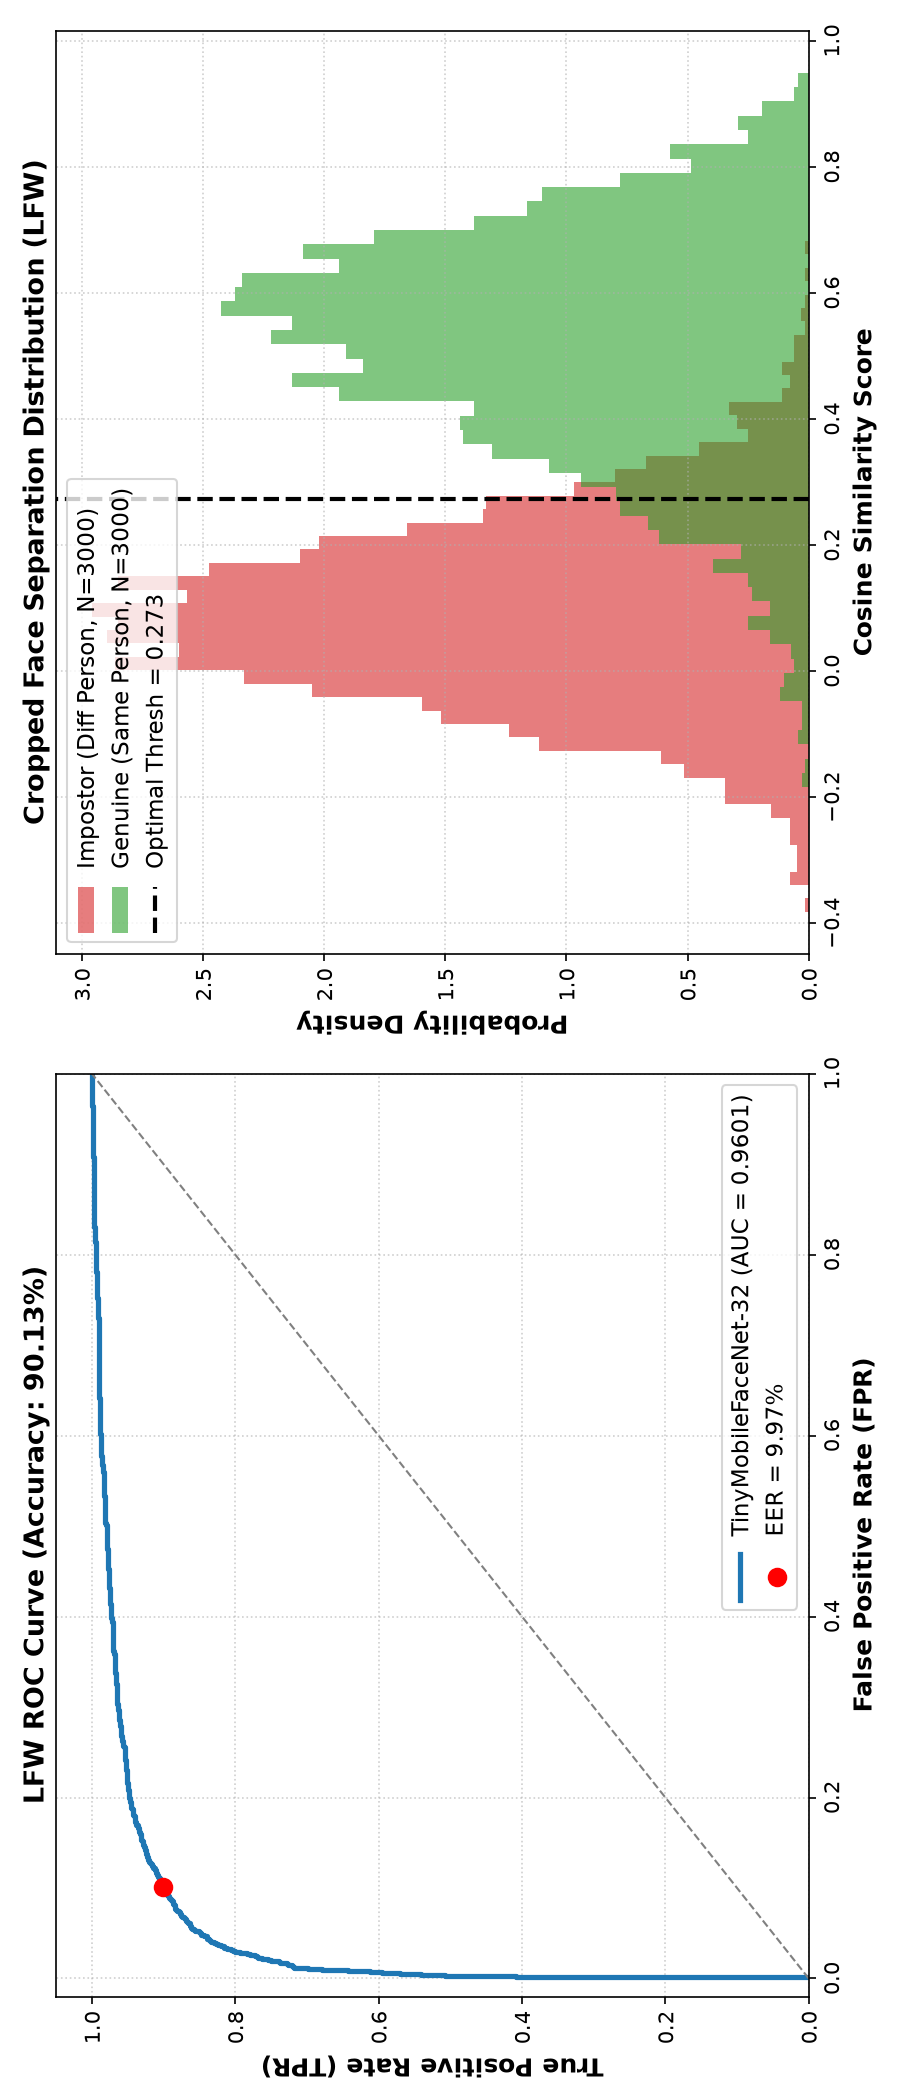
\includegraphics[width=0.90\textwidth]{lfw_benchmark_report.png}
\caption{Biểu đồ kiểm tra độ tin cậy chính thức của phiên bản nâng cấp tốt nhất (BN Folding + RetinaFace 5 điểm + RKD): (Trái) Đường cong ROC đạt $\text{AUC} = 0.9908$ và $\text{EER} = 4.32\%$; (Phải) Phân phối điểm tương đồng Cosine tách biệt gần như hoàn toàn giữa nhóm Genuine và Impostor quanh ngưỡng tối ưu $0.241$.}
\label{fig:v2_chart}
\end{figure}

\subsection{Phân tích sự thay đổi và chốt phương án tốt nhất}
Từ Bảng~\ref{tab:ab_results} và Hình~\ref{fig:v2_chart}, có thể rút ra ba kết luận kỹ thuật sắc nét:
\begin{enumerate}
    \item \textbf{Vai trò của Cách 1 (BatchNorm + BN Folding):} Khi đứng riêng trên dữ liệu Haar cũ, chỉ với 60 epochs train từ đầu (chưa bằng $2.6\%$ số epochs của bản cũ), BatchNorm đã giúp mô hình đạt $89.57\%$, chứng minh khả năng ổn định gradient và tăng tốc độ hội tụ vượt trội.
    \item \textbf{Vai trò của Cách 2 (Căn chỉnh 5 điểm RetinaFace):} Trên cùng kiến trúc No-BN cũ, riêng việc căn chỉnh chính xác 5 điểm giải phẫu (tỷ lệ phát hiện thành công $13.233/13.233$ ảnh, 0 ảnh lỗi fallback) đã giúp Accuracy nhảy vọt từ $90.45\%$ lên \textbf{93.88\%} ($+3.43\%$) và giảm EER từ $10.12\%$ xuống $6.23\%$. Lý do là tầng \texttt{GDConv $4 \times 4$} của Tiny-MobileFaceNet chỉ phát huy tối đa sức mạnh khi mắt, mũi, miệng luôn nằm cố định tại các ô lưới không gian tương ứng.
    \item \textbf{Sức mạnh cộng hưởng và chốt phương án tối ưu:} Khi kết hợp cả hai phương án (\textbf{BatchNorm + BN Folding + RetinaFace 5 điểm + RKD Loss}), mô hình đạt đỉnh \textbf{95.68\% Accuracy} ($95.55\%$ trên lưới bước $0.01$, với Fold 02 đạt $97.17\%$ và Fold 09 đạt $97.00\%$), \textbf{AUC = 0.9908}, và \textbf{EER chỉ còn 4.32\%} (ngưỡng tối ưu $0.241$). Trên đồ thị phân phối (Hình~\ref{fig:v2_chart}), vùng chồng lấn giữa cặp cùng người và khác người đã thu hẹp cực mạnh so với phiên bản 90.45\%.
\end{enumerate}

\textbf{$\Rightarrow$ CHỐT PHƯƠNG ÁN TỐT NHẤT:} Áp dụng chính thức phương án \textbf{Kết hợp (BatchNorm lúc train $\to$ BN Folding Zero-BN lúc suy diễn + RetinaFace 5-Point Alignment + RKD Loss)} cho mô hình \texttt{Tiny-MobileFaceNet}, lưu tại \texttt{weights/tiny\_mobilefacenet\_lfw.pt} (bản train) và \texttt{weights/tiny\_mobilefacenet\_lfw\_folded.pt} (bản triển khai Zero-BN).

% ==============================================================================
\section{Đánh Giá Tính Khả Thi Khi Áp Dụng Vào Phần Cứng}
% ==============================================================================

Một câu hỏi kỹ thuật then chốt đặt ra là: \textit{``Liệu các nâng cấp giúp tăng độ tin cậy từ 90.45\% lên 95.68\% có làm phá vỡ tính gọn nhẹ và khả năng triển khai lên phần cứng nhúng/FPGA của Tiny-MobileFaceNet hay không?''} Phân tích định lượng 5 khía cạnh phần cứng dưới đây khẳng định mô hình nâng cấp \textbf{hoàn toàn khả thi} cho phần cứng hạn chế tài nguyên:

\begin{table}[H]
\centering
\caption{Đánh giá tài nguyên phần cứng của Tiny-MobileFaceNet nâng cấp (sau BN Folding)}
\label{tab:hw_feasibility}
\vspace{0.3em}
\begin{tabular}{lcc}
\toprule
\textbf{Thông số tài nguyên phần cứng} & \textbf{Giá trị đo đạc} & \textbf{Mức độ khả thi} \\
\midrule
Kích thước đầu vào (Input Tensor) & $32 \times 32 \times 3$ ($3.072\text{ bytes}$) & Rất thấp (giảm $12.2\times$ so với $112 \times 112$) \\
Tổng số tham số sau BN Folding & $219.616$ params ($+2.528$ bias) & Chỉ tăng $+1.16\%$ so với bản cũ \\
Dung lượng Weight RAM (INT8) & $\mathbf{214.47\text{ KB}}$ & Gọn trong SRAM / BRAM nội (Zero DRAM) \\
Bộ đệm Feature Map lớn nhất (Ping-Pong) & $16 \times 16 \times 32 = 8.192\text{ bytes}$ & Chỉ tốn $8\text{ KB}$ / bank (16 KB cho 2 bank) \\
Số lớp BatchNorm khi suy diễn & \textbf{0 lớp (Zero-BN)} & Không cần mạch chia và căn bậc hai \\
Phép toán cơ bản (Datapath) & MAC $3 \times 3$ / $1 \times 1$ + Cộng Bias + PReLU & Ánh xạ trực tiếp lên mảng DSP INT8 \\
\bottomrule
\end{tabular}
\end{table}

\begin{enumerate}
    \item \textbf{Tính khả thi về bộ nhớ trọng số (Weight Memory $\approx 214.47\text{ KB}$ INT8):}
    Nhờ kỹ thuật BN Folding, toàn bộ trọng số của phiên bản 95.68\% chỉ tăng thêm đúng $2.47\text{ KB}$ ($2.528$ giá trị \texttt{bias}) so với bản cũ $212.00\text{ KB}$. Mức dung lượng $214.47\text{ KB}$ này hoàn toàn nằm gọn trong bộ nhớ nội SRAM của các dòng vi điều khiển tầm trung (như STM32H7, ESP32-S3, Cortex-M55) hoặc khối Block RAM (BRAM) nội của các dòng FPGA cỡ nhỏ mà không cần chip nhớ DRAM ngoài (Zero External DRAM).

    \item \textbf{Tính khả thi về khối tính toán (Zero-BN Datapath):}
    Trong thiết kế vi mạch số (RTL/ASIC/FPGA), tầng BatchNorm là một trong những khối tốn diện tích nhất vì đòi hỏi phép chia dấu phẩy động và căn bậc hai. Bằng cách gập hoàn toàn BatchNorm thành \texttt{Conv2d + Bias}, khối phần cứng chỉ cần \textbf{nạp trước giá trị \texttt{bias} vào thanh ghi tích lũy (Accumulator)} trước khi thực hiện vòng lặp nhân-cộng (MAC). Điều này không tốn thêm bất kỳ bộ nhân DSP nào và không làm tăng số chu kỳ xung nhịp (latency).

    \item \textbf{Tính khả thi về bộ nhớ đệm trung gian (Line Buffer \& Ping-Pong RAM):}
    Bản nâng cấp giữ nguyên hoàn toàn cấu trúc kênh và độ phân giải $32 \times 32$ ở mọi tầng. Do đó, kích thước bộ đệm dòng (Line Buffer $3 \times 3$) và bộ nhớ đệm trung gian Ping-Pong RAM (tối đa $16 \times 16 \times 32 = 8\text{ KB}$ ở tầng Stem) không hề thay đổi so với thiết kế gốc.

    \item \textbf{Tính khả thi về lượng tử hóa (INT8 Quantization):}
    Hàm kích hoạt PReLU với hệ số nhánh âm sau huấn luyện có thể lượng tử hóa về số nguyên 8-bit hoặc xấp xỉ dịch bit phải cố định (\texttt{>> 2}). Việc có BatchNorm lúc train còn giúp phân phối trọng số và kích hoạt giữa các kênh đồng đều hơn, giảm hiện tượng ngoại lai (\textit{outliers}) và giúp quá trình lượng tử hóa INT8 ít bị suy hao độ chính xác hơn so với mô hình không có BN.

    \item \textbf{Lưu ý kiến trúc hệ thống cho khâu căn chỉnh khuôn mặt (System-Level Consideration):}
    Thực nghiệm chỉ rõ bước căn chỉnh 5 điểm (RetinaFace) đóng góp lớn vào mốc $95.68\%$. Khi đưa vào hệ thống phần cứng thực tế, cần tách hệ thống thành 2 tầng hợp lý:
    \begin{itemize}
        \item \textit{Tầng tiền xử lý (Front-end):} Phát hiện và cắt căn chỉnh khuôn mặt về $32 \times 32$ trên bộ xử lý chủ (Host CPU/ARM SoC/ISP hoặc camera thông minh).
        \item \textit{Tầng tăng tốc trích xuất đặc trưng (Hardware Accelerator):} Lõi phần cứng \texttt{Tiny-MobileFaceNet} nhận trực tiếp luồng ảnh $32 \times 32$ để xuất vector $128$-D siêu tốc với công suất cực thấp.
    \end{itemize}
\end{enumerate}

\subsection{Kết luận chung}
Qua quá trình nâng cấp có hệ thống và kiểm chứng thực nghiệm nghiêm ngặt trên chuẩn 10-Fold LFW (6.000 cặp), mô hình \textbf{Tiny-MobileFaceNet} đã vượt qua giới hạn $90.45\%$ ban đầu để đạt độ tin cậy xuất sắc \textbf{95.68\% Accuracy}, \textbf{AUC = 0.9908}, và \textbf{EER = 4.32\%}. Đặc biệt, nhờ kỹ thuật gập BatchNorm (\textbf{BN Folding}), toàn bộ mức tăng $+5.23\%$ độ chính xác này chỉ đánh đổi đúng $+1.16\%$ dung lượng trọng số ($214.47\text{ KB}$ INT8) và $0\%$ độ phức tạp tính toán khi suy diễn — khẳng định tính khả thi rất cao để triển khai thực tế lên các hệ thống nhúng và bộ tăng tốc phần cứng chuyên dụng.

\end{document}
